\documentclass[dvipdfmx]{article}
\usepackage{tikz}
\usepackage{pgfplots}

\begin{document}

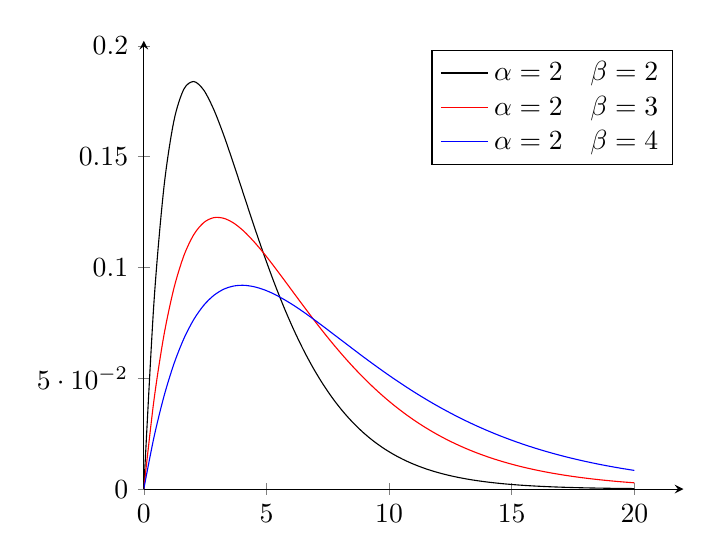
\begin{tikzpicture}[
    declare function={gamma(\z)=
    (2.506628274631*sqrt(1/\z) + 0.20888568*(1/\z)^(1.5) + 0.00870357*(1/\z)^(2.5) - (174.2106599*(1/\z)^(3.5))/25920 - (715.6423511*(1/\z)^(4.5))/1244160)*exp((-ln(1/\z)-1)*\z);},
    declare function={gammapdf(\x,\k,\theta) = \x^(\k-1)*exp(-\x/\theta) / (\theta^\k*gamma(\k));}
]

\begin{axis}[
    axis lines=left,
    enlargelimits=upper,
    samples=50,
    legend entries={$\alpha=2\quad \beta=2$, $\alpha=2\quad \beta=3$, $\alpha=2\quad \beta=4$}
]
\addplot [smooth, domain=0:20] {gammapdf(x,2,2)};
\addplot [smooth, domain=0:20, red] {gammapdf(x,2,3)};
\addplot [smooth, domain=0:20, blue] {gammapdf(x,2,4)};
\end{axis}

\end{tikzpicture}

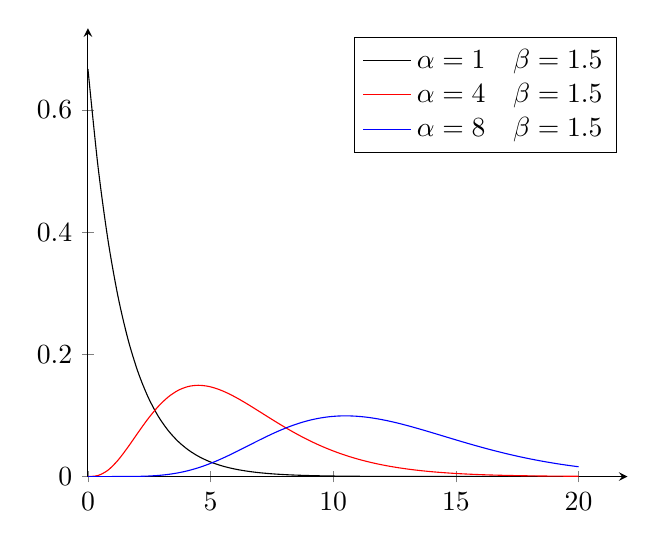
\begin{tikzpicture}[
    declare function={gamma(\z)=
    (2.506628274631*sqrt(1/\z) + 0.20888568*(1/\z)^(1.5) + 0.00870357*(1/\z)^(2.5) - (174.2106599*(1/\z)^(3.5))/25920 - (715.6423511*(1/\z)^(4.5))/1244160)*exp((-ln(1/\z)-1)*\z);},
    declare function={gammapdf(\x,\k,\theta) = \x^(\k-1)*exp(-\x/\theta) / (\theta^\k*gamma(\k));}
]

\begin{axis}[
    axis lines=left,
    enlargelimits=upper,
    samples=50,
    legend entries={$\alpha=1\quad \beta=1.5$, $\alpha=4\quad \beta=1.5$, $\alpha=8\quad \beta=1.5$}
]
\addplot [smooth, domain=0:20] {gammapdf(x,1,1.5)};
\addplot [smooth, domain=0:20, red] {gammapdf(x,4,1.5)};
\addplot [smooth, domain=0:20, blue] {gammapdf(x,8,1.5)};
\end{axis}
\end{tikzpicture}
\end{document}